% !TEX TS-program = XeLaTeX
% !TeX root=main.tex
% در این فایل، عنوان پایان‌نامه، مشخصات خود، متن تقدیمی ، ستایش، سپاس گزاری و چکیده پایان‌نامه را به فارسی، وارد کنید.
% توجه داشته باشید که جدول حاوی مشخصات پروژه/پایان‌نامه/رساله و همچنین، مشخصات داخل آن، به طور خودکار، درج می‌شود.
%%%%%%%%%%%%%%%%%%%%%%%%%%%%%%%%%%%%
% دانشگاه خود را وارد کنید
\university{حکیم سبزواری}
% دانشکده، آموزشکده و یا پژوهشکده  خود را وارد کنید
\faculty{دانشکده ریاضی و علوم کامپیوتر}
% گروه آموزشی خود را وارد کنید - فعلاً فعال نیست
%\department{ریاضی کاربردی}
% رشته خود را وارد کنید
\subject{ریاضی کاربردی}
% گرایش خود را وارد کنید
\field{تحقیق در عملیات}
% عنوان پایان‌نامه را وارد کنید
\title{نوشتن پروژه، پایان‌نامه و رساله با استفاده از کلاس 
HSU-Thesis ( نسخه ۱.۵)}
% نام استاد(ان) راهنما را وارد کنید
\firstsupervisor{دکتر مهدی زعفرانیه}
%\secondsupervisor{دکتر وفا خلیقی}
% نام استاد(دان) مشاور را وارد کنید. چنانچه استاد مشاور ندارید، دستورات پایین را غیرفعال کنید.
\firstadvisor{دکتر علیرضا قدسی}
%\secondadvisor{وحید دامن افشان}
% نام دانشجو را وارد کنید
\name{محمود}
% نام خانوادگی دانشجو را وارد کنید
\surname{امین‌طوسی}
% شماره دانشجویی دانشجو را وارد کنید
\studentID{89922012}
% تاریخ پایان‌نامه را وارد کنید
\thesisdate{شهریور ۱۳۹۵}
% به صورت پیش فرض برای پایان‌نامه‌های کارشناسی تا دکترا به ترتیب از عبارات «پروژه»، «پایان‌نامه» و »رساله» استفاده می‌شود؛ اگر  نمی پسندید هر عنوانی را که مایلید در دستور زیر قرار داده و آنرا از حالت توضیح خارج کنید.
%\projectLabel{پایان‌نامه}

% به صورت پیش فرض برای عناوین مقاطع تحصیلی کارشناسی تا دکترا به ترتیب از عبارات «کارشناسی»، «کارشناسی ارشد» و »دکترا» استفاده می‌شود؛ اگر  نمی پسندید هر عنوانی را که مایلید در دستور زیر قرار داده و آنرا از حالت توضیح خارج کنید.
%\degree{}

% در این قسما اسامی داوران، نماینده تحصیلات تکمیلی و مدیر گروه را بنویسید.
\firstReviewer{دکتر علی‌اصغر مولوی}
%\secondReviewer{داور۲}
%\thirdReviewer{داور۳}
\representative{دکتر غلامرضا مقدسی}
\departmentHead{دکتر محمدعلی پرتانیان}


% کلمات کلیدی پایان‌نامه را وارد کنید
\keywords{زی‌پرشین، لاتک، قالب پایان‌نامه، الگو}
%چکیده پایان‌نامه را وارد کنید، برای ایجاد پاراگراف جدید از \\ استفاده کنید. اگر خط خالی دشته باشید، خطا خواهید گرفت.
\faAbstract{
این پایان‌نامه، به بحث در مورد نوشتن پروژه، پایان‌نامه و رساله با استفاده از کلاس 
\lr{HSU-Thesis}
می‌پردازد.
حروف‌چینی پروژه کارشناسی، پایان‌نامه یا رساله یکی از موارد پرکاربرد استفاده از لاتک است. 
از جمله مزایای لاتک آن است که در صورت وجود یک کلاس آماده برای حروف‌چینی یک سند خاص مانند یک پایان‌نامه، کاربر بدون درگیری با جزییات حروف‌چینی و صفحه آرایی می تواند سند خود را آماده نماید.
\\
شاید با قالب های لاتکی که برخی از مجلات برای مقالات خود عرضه می‌کنند مواجه شده باشید. اگر نظیر این کار در دانشگاههای مختلف برای اسناد متنوع آنها مانند پایا ن نامه‌ها آماده شود، دانشجویان به جای وقت گذاشتن روی صفحه آرایی مطالب خود، روی محتوای متن خود تمرکز خواهند نمود. به علاوه با آشنایی با لاتک خواهند توانست از امکانات بسیار این نرم افزار جهت نمایش بهتر دست آوردهای خود استفاده کنند.
به همین خاطر، یک کلاس با نام 
\lr{HSU-Thesis}
 برای حروف‌چینی پروژه‌ها، پایان‌نامه‌ها و رساله‌های دانشگاه حکیم سبزواری با استفاده از لاتک آماده شده است که مطابق با الگوی مورد تایید مدیریت تحصیلات تکمیلی دانشگاه حکیم سبزواری می‌باشد.
}
 % پایان‌نامه خود را تقدیم نموده و از افرادی که در این مسیر به شما یاری رسانده‌اند سپاس‌گزاری نمایید!
% درصورتی که به‌ بخش تقدیم نیاز ندارید، کل بخش زیر را حذف کنید یا به حالت توضیح درآورید.
\faDedication
{
\begin{flushright}
{\Large تقدیم به:}
\end{flushright}
\begin{center}
{\huge
همسر و فرزندانم\\
و\\
\vspace{7mm}
پدر و مادرم
}
\end{center}
}

% سپاس گزاری، دقت داشته باشید که در داخل این قسمتها نمی‌توانید خط خالی رد کنید و درصورت نیاز به رفتن به خط بعد باید از \\ استفاده کنید.
% درصورتی که به‌ قسمت قدردانی نیاز ندارید، کل بخش زیر را حذف کنید یا به حالت توضیح درآورید.
\faAcknowledgement{
سپاس خداوندگار حکیم را که با لطف بی کران خود، آدمی را زیور عقل آراست.\\
در آغاز وظیفه   خود  می دانم از زحمات بی دریغ استاد  راهنمای خود،  جناب آقای دکتر ...، صمیمانه تشکر و  قدردانی کنم  که قطعاً بدون راهنمایی های ارزنده   ایشان، این مجموعه  به انجام  نمی رسید.\\
از جناب  آقای  دکتر ...   که زحمت  مطالعه و مشاوره   این رساله را تقبل  فرمودند و در آماده سازی  این رساله، به نحو احسن اینجانب را مورد راهنمایی قرار دادند، کمال امتنان را دارم.\\
همچنین لازم می دانم از گروه پارسی‌لاتک در پاسخگویی به مشکلات کاربران کمال قدردانی را داشته باشم.\\
 در پایان، بوسه می زنم بر دستان خداوندگاران مهر و مهربانی، پدر و مادر عزیزم و بعد از خدا، ستایش می‌کنم وجود مقدس شان را و تشکر می‌کنم از خانواده عزیزم به پاس عاطفه سرشار و گرمای امیدبخش وجودشان، که بهترین پشتیبان من بودند.
}


\firstPage

% رفع مشکل عدم نمایش فهرست الگوریتم‌ها
\renewcommand{\listofalgorithms}{\begingroup
\tocfile{فهرست الگوریتم‌ها}{loa}
\endgroup}
\makeatletter
\let\l@algorithm\l@figure
\makeatother


% بررسی حالت پیش‌نویس
\ifoptiondraft{}{% 
% درج صفحه فرم ارزشیابی و صورتجلسه دفاع، به همراه مشخصات داوران
\davaranPage 
% اگر مایلید صورتجلسه دفاع اسکن شده را به جای آن قرار دهید، خط بالا را در حالت توضیح قرار دهید، دستور زیر را فعال کنید و نام فایل اسکن شده را داخل آکولاد بنویسید.
%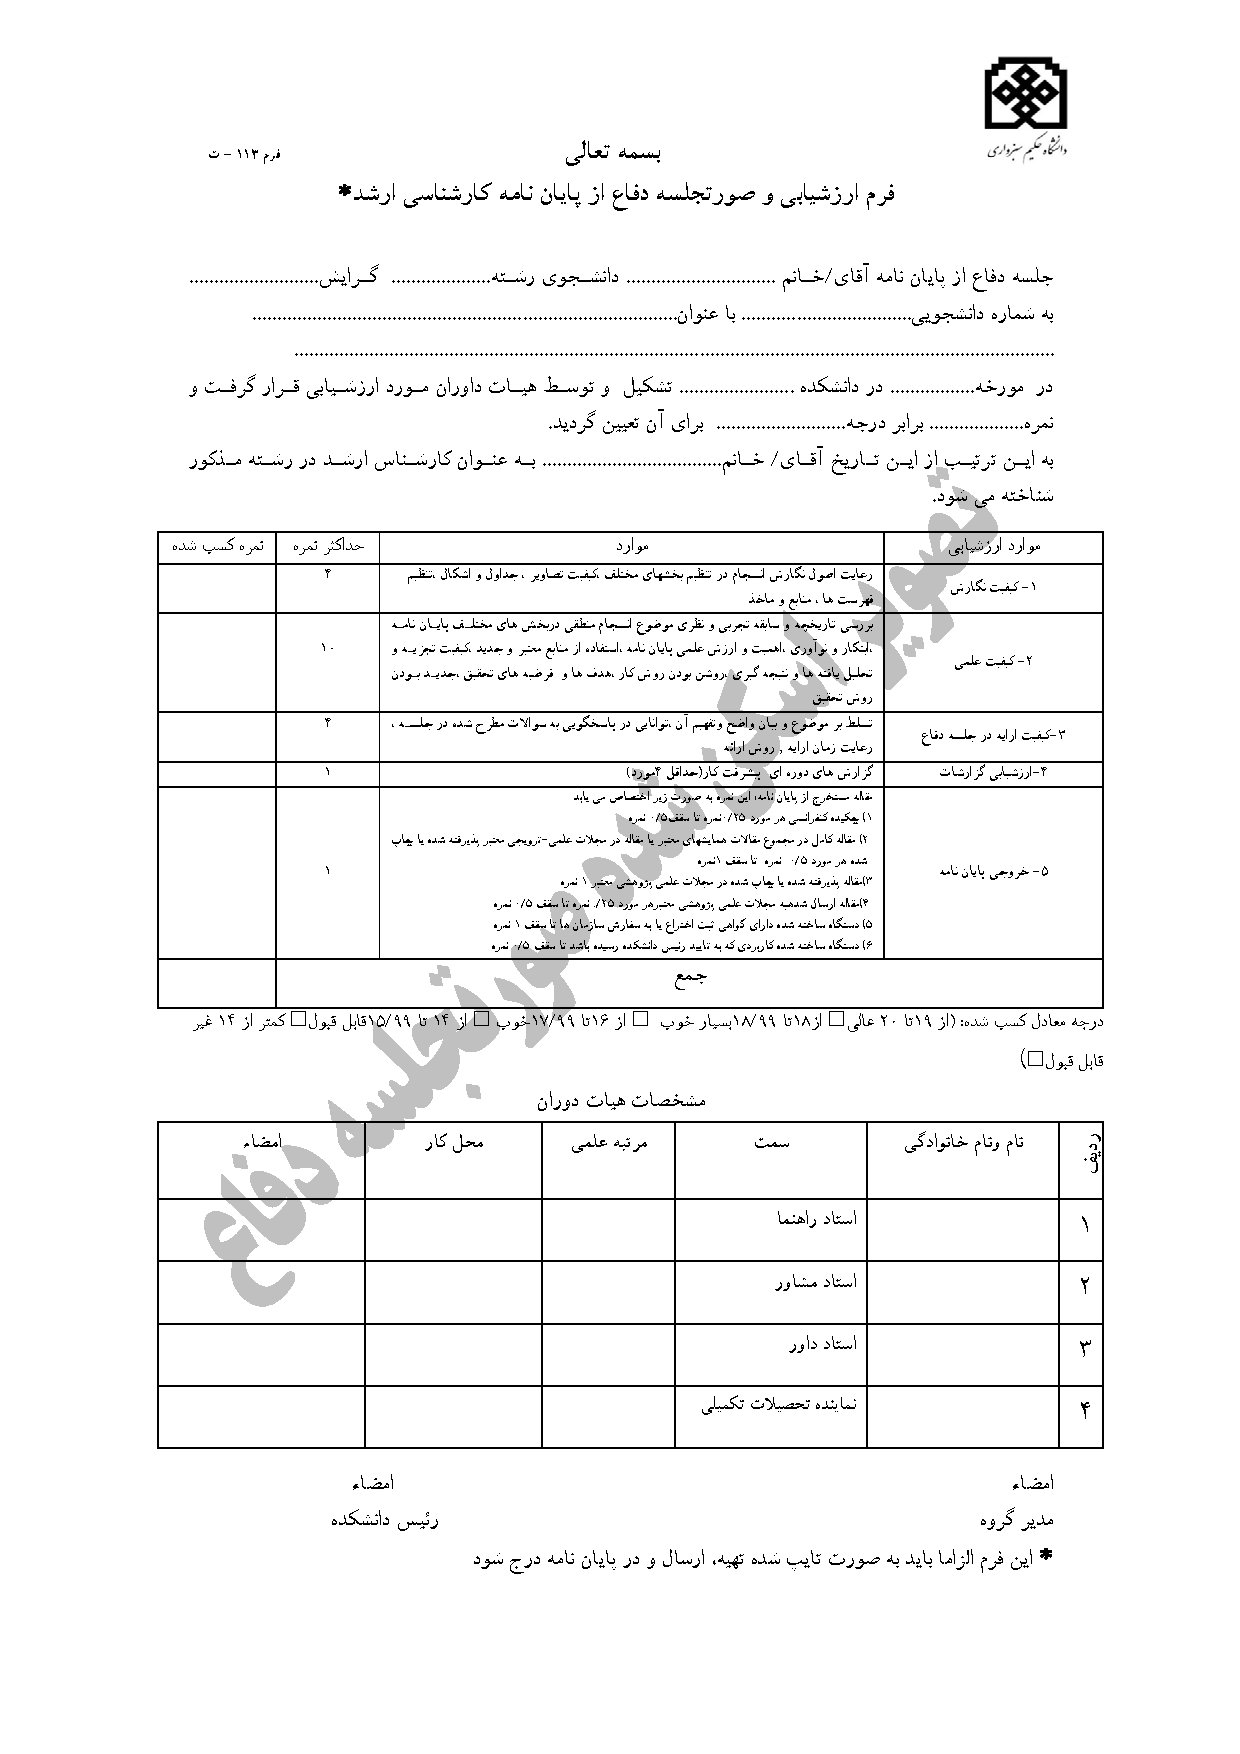
\includepdf{sooratjalaseh.pdf}

\doublespacing
\sogandPage
\esalatPage
\mojavezPage % اگر صفحه مجوز بهره برداری را نمیخواهید این خط را در حالت توضیح قرار دهید.
\sepasPage
} % end ifoptiondraft

\newpage\clearpage

\pagenumbering{alph}
\tableofcontents

\ifoptiondraft{
\setcounter{tocdepth}{1}
\listoftodos
\pagestyle{plain}
\pagenumbering{arabic}
}{%
% اگر مایلید فهرست  کلمات اختصاری را داشته باشید خط زیر را از حالت توضیح خارج کنید و کلمات خود را داخل فایل acronyms بنویسید.
%\newpage % !TEX TS-program = XeLaTeX
% !TeX root=main.tex
\chapter*{فهرست علائم اختصاری}
\addcontentsline{toc}{chapter}{فهرست علائم اختصاری}

\persiangloss{شتاب گرانش}{$a$ (m/s$^2$)}
\persiangloss{نیرو}{$F$ (N)}

\newpage \listoftables  
\newpage \listoffigures 

% اگر مایلید فهرست الگوریتمها را داشته باشید خطوط زیر را از حالت توضیح خارج کنید.
%\newpage
%\listofalgorithms 


\pagestyle{plain}
\clearpage
\pagenumbering{arabic}

\newpage
\abstractPage
}
